\chapter{Setup dos Serviços}

Nesta secção são abordadas a alocação e configuração dos diferentes serviços nos diferentes computadores.

A tipologia de rede usada foi a seguinte:

\begin{table}[H]
    \begin{center}
        \begin{tabular}{ || c | c ||}
        \hline
        \textbf{Serviço} & \textbf{Computador}\\ 
        \hline
        HTTP Server & Tux14\\ 
        \hline
        DNS Server & Tux14\\ 
        \hline
        FTP Server & Tux12\\ 
        \hline
        NTP Server & Tux12\\ 
        \hline
        Email Server & Tux12 / Tux14\\ 
        \hline
        SNMP & Router / Switch\\ 
        \hline
        Nagios & Tux13\\
        \hline
        Zabbix & Tux13\\
        \hline
        \end{tabular}
    \end{center}
    \caption{Alocação dos serviços nos computadores}
    \label{tab:ip_table}
\end{table}

Todos os serviços instalados serão mencionados e testados, no entanto as suas instalações não serão abordadas dado que são iguais aos trabalhos anteriores.


%%%%%%%%%%%%%%%%%%%%%%%%%%%%%%%%%%%%%%%%%%%%%%%%%%%%%%%%%%%%%%%%%%%%%%%%%%%%%%%%%%%%%%%
\section{HTTP Server}

O servidor HTTP foi configurado com recurso ao \textbf{Apache} \cite{Apache}.
Este servidor corre uma página dinâmica PHP para impedir \textit{caching} do seu conteúdo.

\begin{figure}[H]
    \centering
    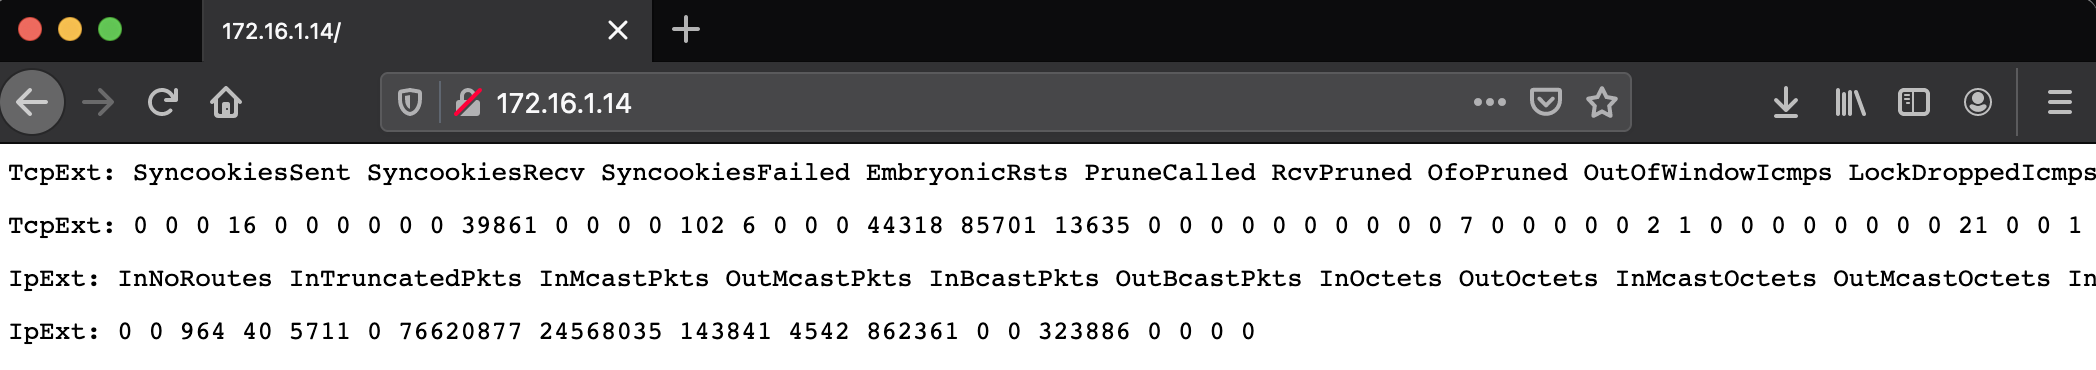
\includegraphics[width=.8\linewidth]{figs/setup/apache}
    \caption{Servidor Apache no Tux14}
    \label{fig:apache_setup}
\end{figure}

\pagebreak

%%%%%%%%%%%%%%%%%%%%%%%%%%%%%%%%%%%%%%%%%%%%%%%%%%%%%%%%%%%%%%%%%%%%%%%%%%%%%%%%%%%%%%%
\section{DNS Server}

O servidor DNS foi configurado com recurso ao \textbf{Bind} \cite{Bind}.
No servidor DNS foi configurado como \textbf{Cache DNS}, fazendo \textit{forward} para endereços que não consegue resolver para
os servidores DNS da \textit{Google}.
Na base de dados local foi adicionada a entrada do domínio \verb|www.example.com|, com o respetivo IP \verb|172.16.1.15|.

\begin{figure}[H]
    \centering
    \begin{subfigure}[b]{0.49\textwidth}
        \centering
        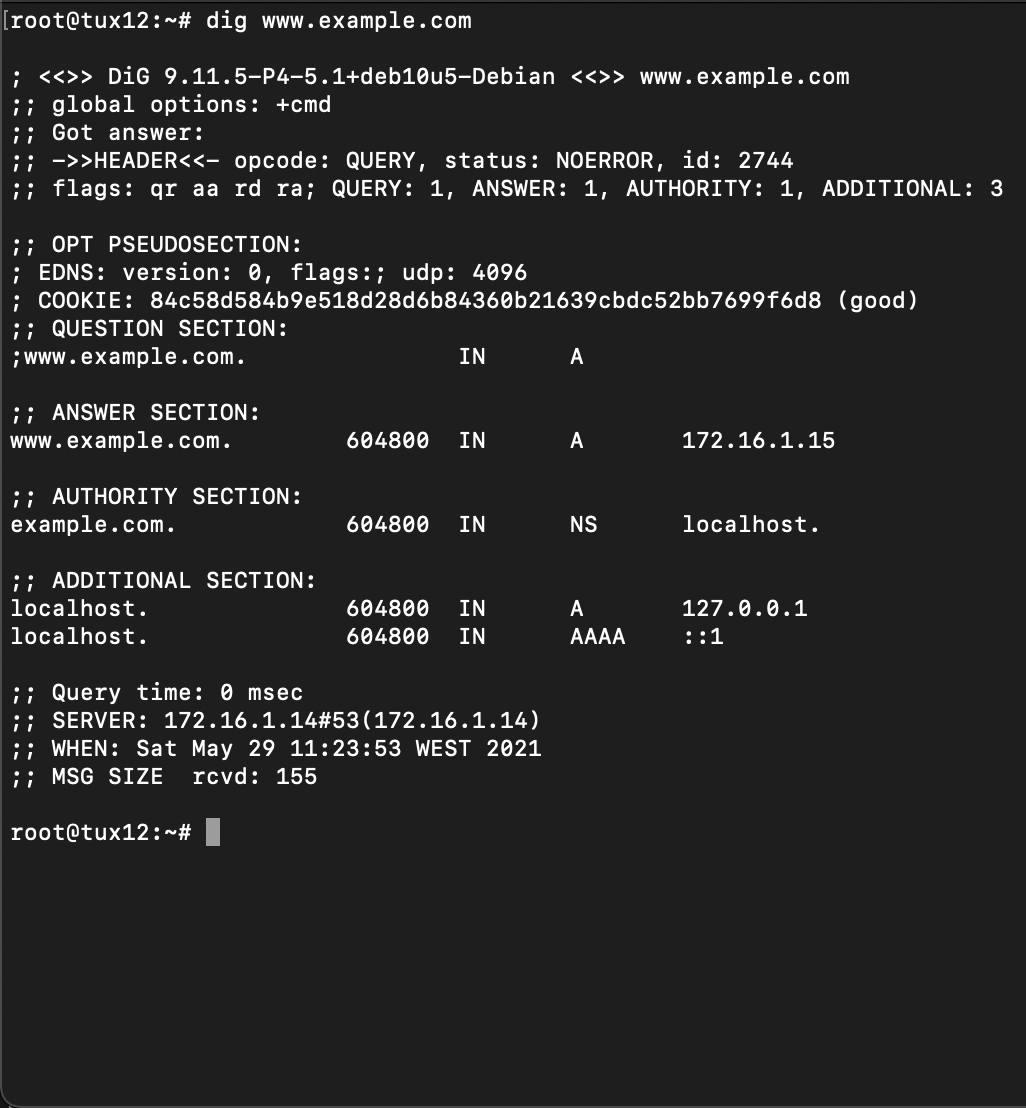
\includegraphics[width=.9\linewidth,height=\textwidth]{figs/setup/dns_example}
        \caption{Resolução do endereço www.example.com}
        \label{fig:dns_example}
    \end{subfigure}
    \hfill
    \begin{subfigure}[b]{0.49\textwidth}
        \centering
        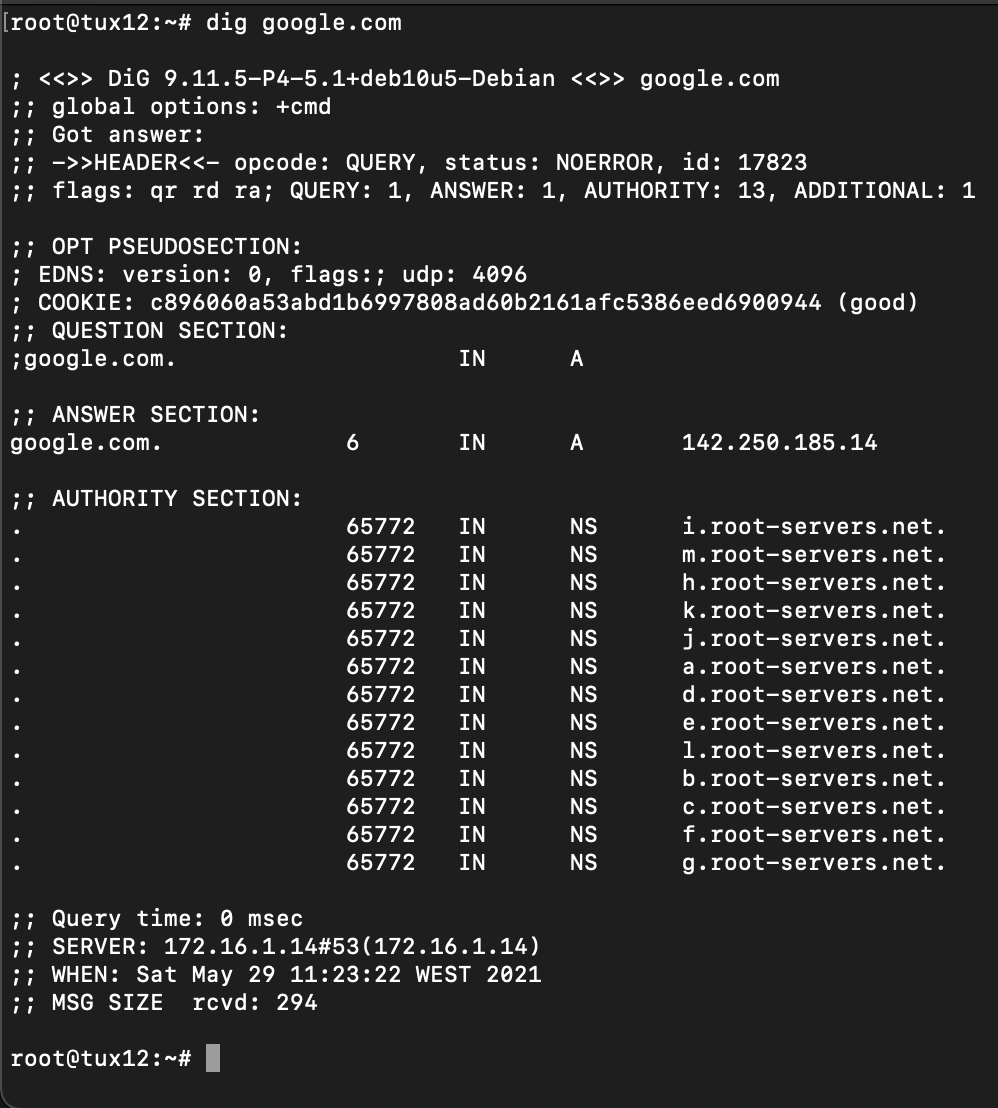
\includegraphics[width=.9\linewidth,height=\textwidth]{figs/setup/dns_cache}
        \caption{Caching da queries}
        \label{fig:dns_cache}
    \end{subfigure}
    \caption{}
\end{figure}

%%%%%%%%%%%%%%%%%%%%%%%%%%%%%%%%%%%%%%%%%%%%%%%%%%%%%%%%%%%%%%%%%%%%%%%%%%%%%%%%%%%%%%%
\section{NTP Server}

O servidor NTP foi configurado com recurso ao \textit{daemon} NTP \cite{NTP}.
Para sincronização, foram definidos os 3 servidores NTP indicados para Portugal \url{https://support.ntp.org/bin/view/Servers/NTPPoolServers}.
O servidor está alojado no \textit{tux12}, mas um cliente foi criado no \textit{tux13} para efeitos de teste.

\begin{figure}[H]
    \centering
    \begin{subfigure}[b]{0.9\textwidth}
        \centering
        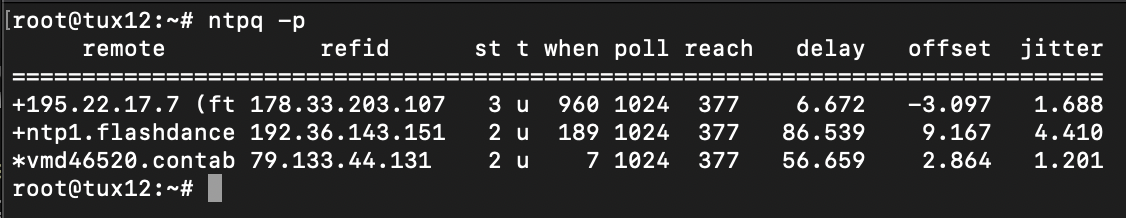
\includegraphics[width=.9\linewidth]{figs/setup/ntp_server}
        \caption{Resolução do endereço www.example.com}
        \label{fig:ntp_server}
    \end{subfigure}
    \hfill
    \begin{subfigure}[b]{0.9\textwidth}
        \centering
        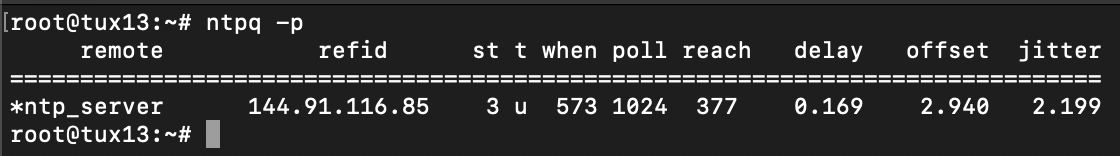
\includegraphics[width=.9\linewidth]{figs/setup/ntp_client}
        \caption{Caching da queries}
        \label{fig:ntp_clinte}
    \end{subfigure}
    \caption{}
\end{figure}

\pagebreak

%%%%%%%%%%%%%%%%%%%%%%%%%%%%%%%%%%%%%%%%%%%%%%%%%%%%%%%%%%%%%%%%%%%%%%%%%%%%%%%%%%%%%%%
\section{FTP Server}

O servidor FTP foi configurado com recurso ao \textbf{vsftpd} \cite{FTP}.
Foram definidos os dados de autenticação e colocado um ficheiro txt para efeitos de teste.

\begin{figure}[H]
    \centering
    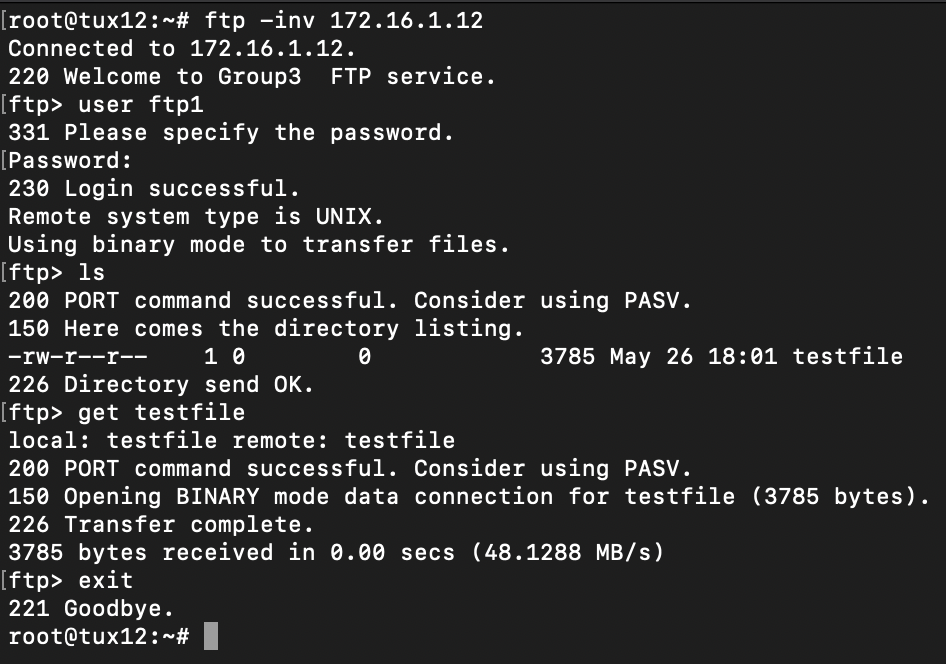
\includegraphics[width=.8\linewidth]{figs/setup/ftp_setup}
    \caption{Acesso ao servidor FTP}
    \label{fig:ftp_setup}
\end{figure}

%%%%%%%%%%%%%%%%%%%%%%%%%%%%%%%%%%%%%%%%%%%%%%%%%%%%%%%%%%%%%%%%%%%%%%%%%%%%%%%%%%%%%%%
\section{SNMP}

De modo a monitorizar o estado do \textbf{Switch} e do \textbf{Router}, foi ativado um agente SNMP nestes dispositivos \cite{SNMP}.
Este agente permite que, com recurso a este protocolo, uma ferramenta de monitorização tenha acesso a um conjunto de estatísticas que definem o estado do dispositivo. 

Para ativar o SNMP, foi executado o comando \verb|snmp-server community public ro| com permissões apenas de leitura das variáveis.

\pagebreak

%%%%%%%%%%%%%%%%%%%%%%%%%%%%%%%%%%%%%%%%%%%%%%%%%%%%%%%%%%%%%%%%%%%%%%%%%%%%%%%%%%%%%%%
\section{Email Server}
Dois servidores email forma configurados com recurso ao \textbf{Postfix} \cite{Email}.
Foram configurados dois servidores para permitir testar o serviço enviando emails de um servidor para o outro.

\begin{figure}[H]
    \centering
    \begin{subfigure}[b]{0.9\textwidth}
        \centering
        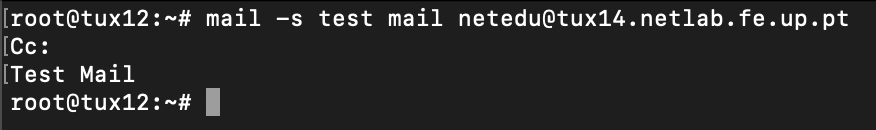
\includegraphics[width=.8\linewidth]{figs/setup/mail_send}
        \caption{Envio de email do Tux12 para Tux14}
        \label{fig:mail_send}
    \end{subfigure}
    \hfill
    \begin{subfigure}[b]{0.9\textwidth}
        \centering
        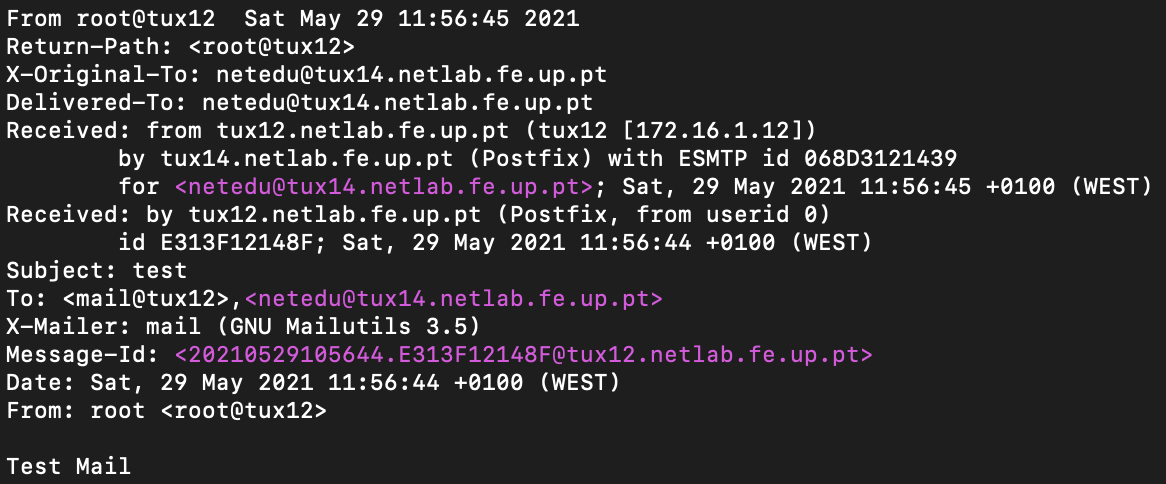
\includegraphics[width=.8\linewidth]{figs/setup/mail_receive}
        \caption{Receção do email no Tux14}
        \label{fig:mail_receive}
    \end{subfigure}
    \caption{}
\end{figure}